\begin{frame}
\frametitle{Aufgabe 1}
\framesubtitle{Bestimmung von komplexem Widerstand und Phase}
    \begin{itemize}
        \item Bestimmung des Widerstands durch Messung von Strom und Spannung
        \item Strommessung = Spannungsmessung an bekanntem Widerstand
    \end{itemize}    
    \begin{figure}[H]
    \begin{center}
            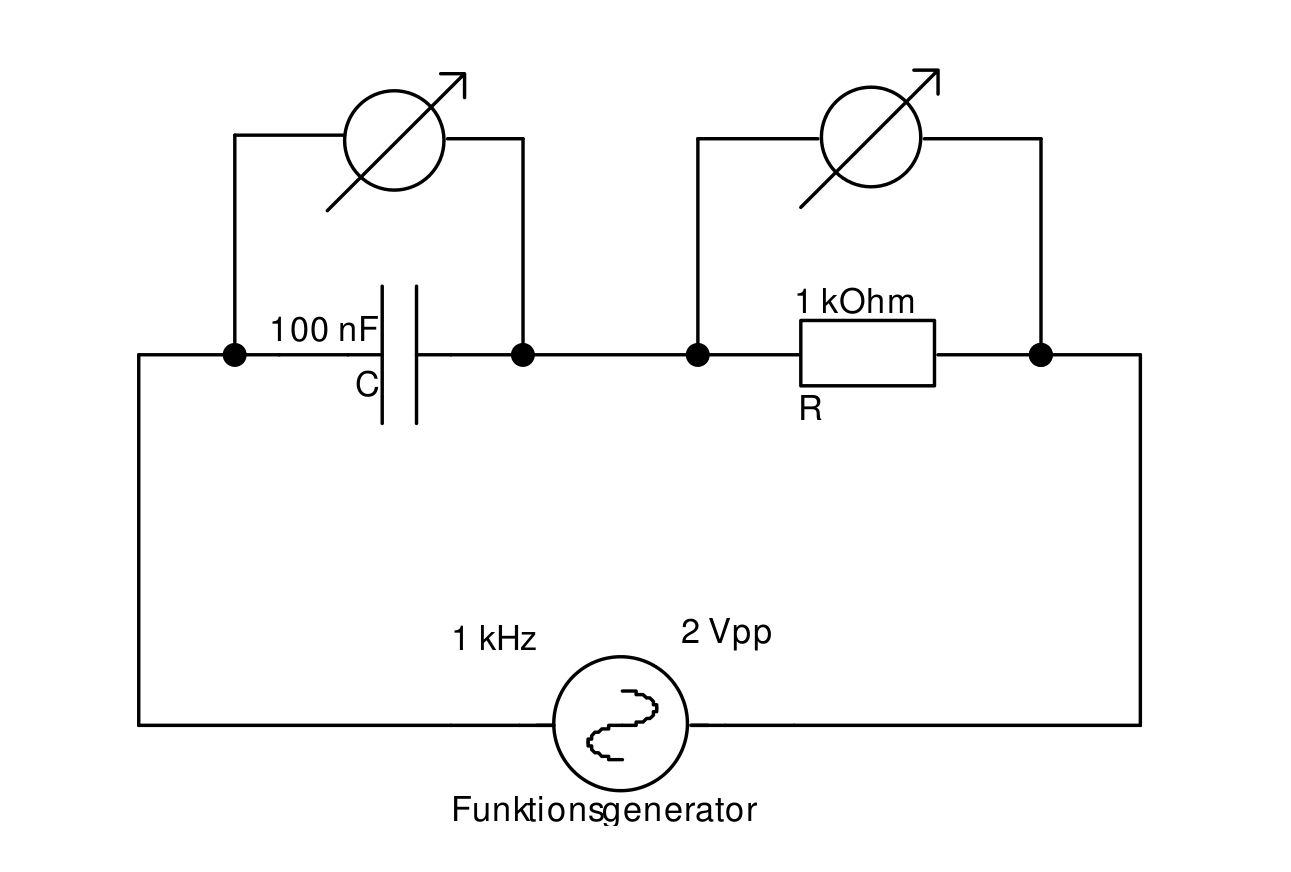
\includegraphics[scale=0.15]{./img/schaltbild_1_ohne_erdung.png}
    \end{center}
    \end{figure}
\end{frame}
\begin{frame}
\frametitle{Aufgabe 1}
\framesubtitle{Bestimmung von komplexem Widerstand und Phase}
    \begin{itemize}
        \item Problem: Erdschleife
    \end{itemize}
    %\begin{figure}[H]
    %\begin{center}
    %        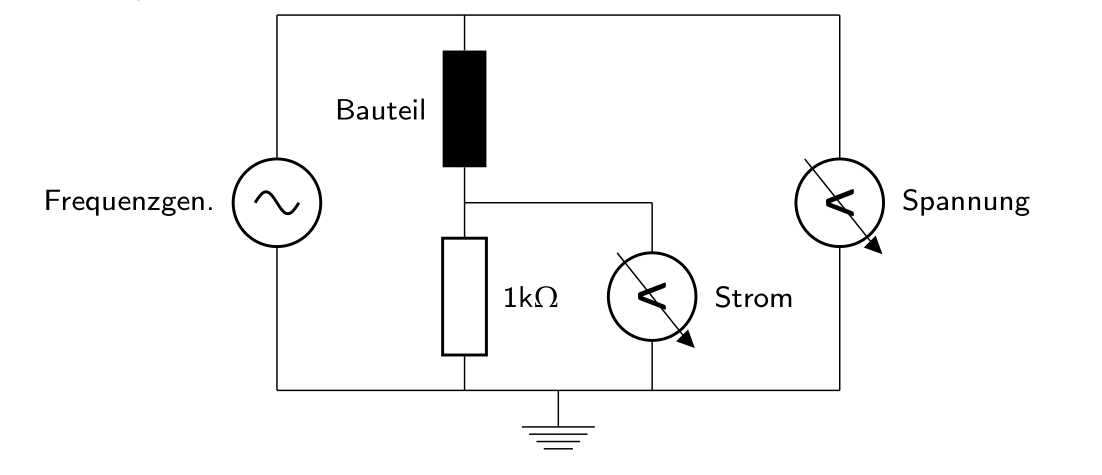
\includegraphics[scale=0.15]{./img/schaltbild_1_mit_erdschleife.png}
    %\end{center}
    %\end{figure}
\end{frame}
\begin{frame}
\frametitle{Aufgabe 1}
\framesubtitle{Bestimmung von komplexem Widerstand und Phase}
    \begin{itemize}
        \item Problem: Erdschleife
        \item Lösung: Erdungen aufeinander legen
        \item Abfall über Bauteil: "Math function 1 - 2"
    \end{itemize}
    %\begin{figure}[H]
    %\begin{center}
    %        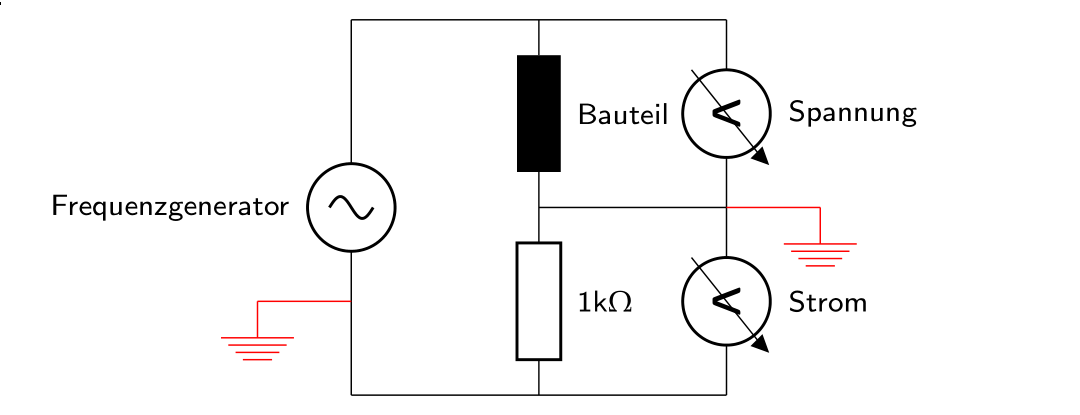
\includegraphics[scale=0.15]{./img/schaltbild_1_alle_erdungen.png}
    %\end{center}
    %\end{figure}
\end{frame}

\begin{frame}
\frametitle{Aufgabe 1}
\framesubtitle{Kondensator}
\begin{figure}[H]
    \begin{center}
                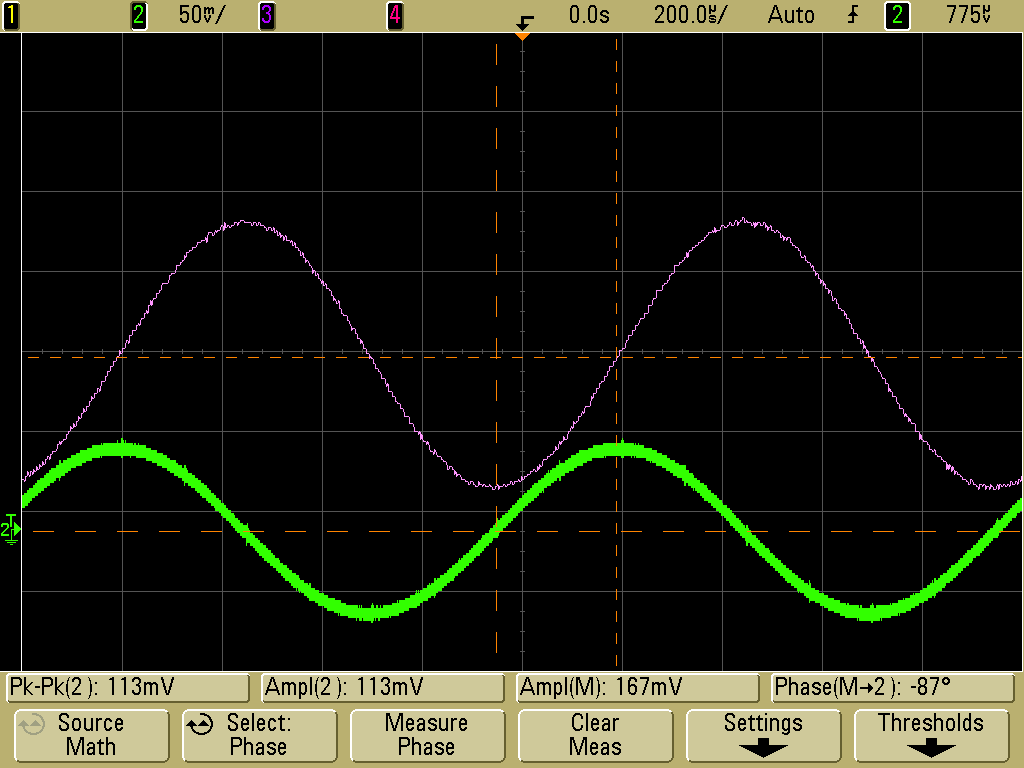
\includegraphics[scale=0.15]{./img/1a_Kondensator_1.png}
    \end{center}
\end{figure}
\begin{center}
\begin{tabular}{c|| c | c | c}
    & $I$ & $U$ & $\varphi$ \\
    \hline
    Kondensator & $113 \mu A$ & $167mV$ & $-87^{\circ}$ \\
\end{tabular}
\end{center}
\end{frame}

\begin{frame}
\frametitle{Aufgabe 1}
\framesubtitle{Spule}
\begin{figure}[H]
    \begin{center}
                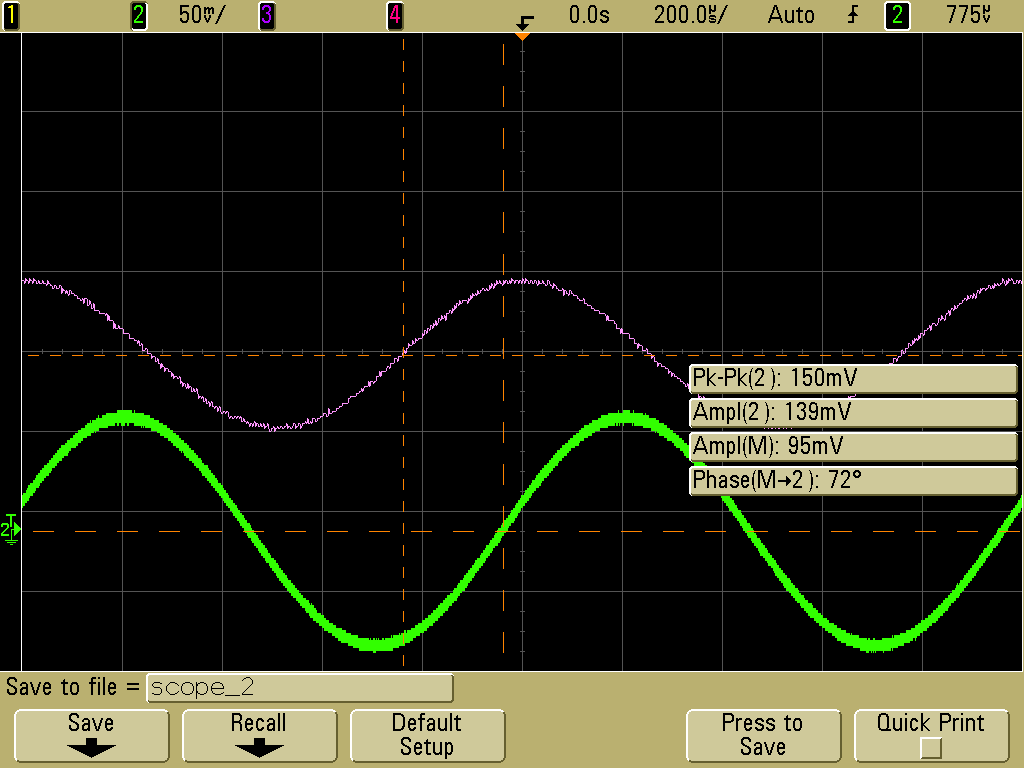
\includegraphics[scale=0.15]{./img/1b_Spule.png}
    \end{center}
\end{figure}
\begin{center}
\begin{tabular}{c|| c | c | c}
    & $I$ & $U$ & $\varphi$ \\
    \hline
    Kondensator & $113 \mu A$ & $167mV$ & $-87^{\circ}$ \\
    Spule & $139 \mu A$ & $95 mV$ & $72^{\circ}$ 
\end{tabular}
\end{center}
\end{frame}

\begin{frame}
\frametitle{Aufgabe 1}
\framesubtitle{Widerstand}
\begin{figure}[H]
    \begin{center}
                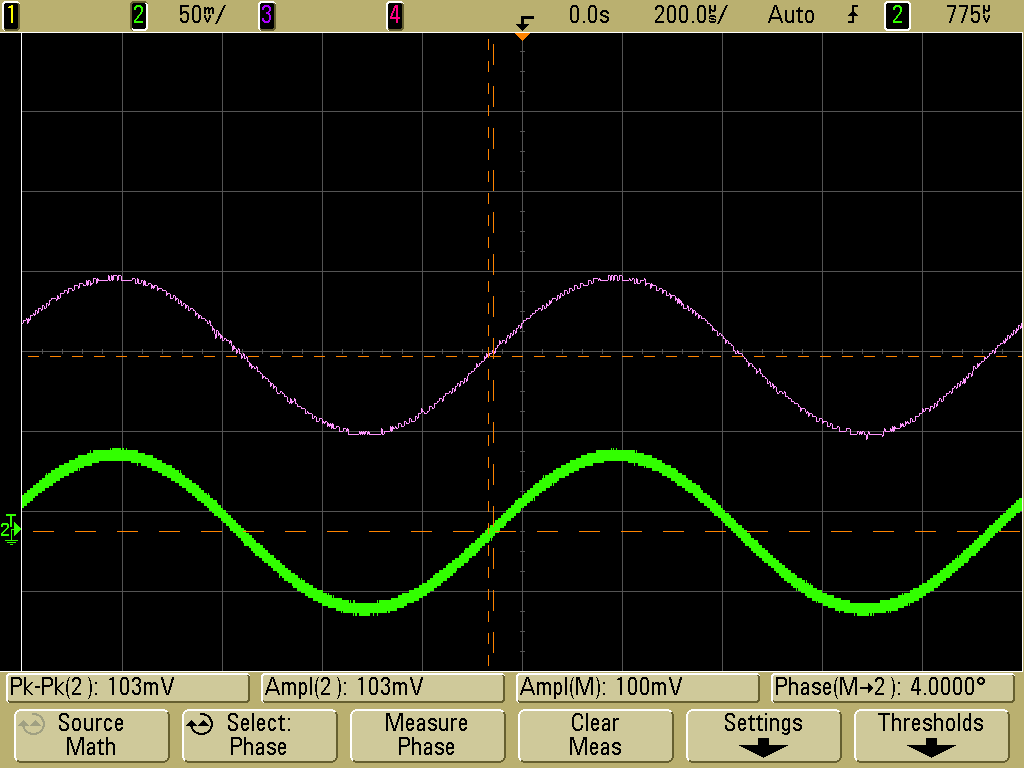
\includegraphics[scale=0.15]{./img/1c_Widerstand.png}
    \end{center}
\end{figure}
\begin{center}
\begin{tabular}{c|| c | c | c}
    & $I$ & $U$ & $\varphi$ \\
    \hline
    Kondensator & $113 \mu A$ & $167mV$ & $-87^{\circ}$ \\
    Spule & $139 \mu A$ & $95 mV$ & $72^{\circ}$  \\
    Widerstand & $104 \mu A$ & $100 mV$ & $4^{\circ}$
\end{tabular}
\end{center}
\end{frame}
\begin{frame}
\frametitle{Aufgabe 1}
\framesubtitle{Auswertung}
\begin{itemize}
    \item Komplexer Widerstand: $Z = \frac{U}{I} \left( \cos (\varphi) + i \sin
    (\varphi) \right) $
\end{itemize}
\begin{align*}
    Z_C &\approx 77.35 - i475.85 \Omega \\
    Z_L &\approx 211.20 - i650.00 \Omega \\
    Z_R &\approx 968.51 - i 67.72 \Omega 
\end{align*}
\pause
\begin{itemize}
    \item $C = -i \frac{1}{2\pi f Z_C}$ und $L = \frac{Z_L}{i2\pi f}$:
\end{itemize}
\begin{align*}
    C &\approx 108 - i5.64nF \\
    L &\approx 103.45 - i33.61 mH
\end{align*}
\end{frame}
\begin{frame}
\frametitle{Aufgabe 1}
\framesubtitle{Auswertung}
\begin{center}
    \begin{tabular}{c|c|c}
        & Theorie & Messung \\
        \hline
        $\varphi_C$ & $-90^{\circ}$ & $-87^{\circ} $\\
        $\varphi_L$ & $90^{\circ}$ & $72^{\circ} $\\
        $\varphi_R$ & $0^{\circ}$ & $4^{\circ} $
    \end{tabular}
\end{center}
\begin{itemize}
    \item Gründe für Abweichung:
    \begin{itemize}
        \item ohmscher Widerstand der Bauteile
        \item Widerstand in Messgeräten
        \item Messungenauigkeit
    \end{itemize}
\end{itemize}
\end{frame}
